\section[Introdução]{Introdução}

Atualmente, o transporte escolar carece de soluções tecnológicas dedicadas,
sendo gerido, em sua maioria, de forma manual ou por meio de ferramentas
improvisadas. Essa lacuna dificulta o controle de passageiros e a logística de rotas,
resultando em ineficiências e falta de transparência.
Este projeto propõe o desenvolvimento de um sistema Web responsivo
(focado em dispositivos móveis) projetado para otimizar a gestão operacional dos
motoristas e elevar o padrão de segurança. A plataforma permitirá o monitoramento
de trajetos em tempo real, o registro de métricas e a comunicação direta com os
responsáveis. O objetivo central é reduzir custos operacionais e oferecer uma
experiência confiável e transparente para as famílias.
O projeto conta com uma equipe de 18 desenvolvedores em fases diversas
do curso, orientados pela professora Ana Paula Bacelo.

\begin{figure}[H]
    \centering
    \small
    \caption{Time do Projeto VanGO}
    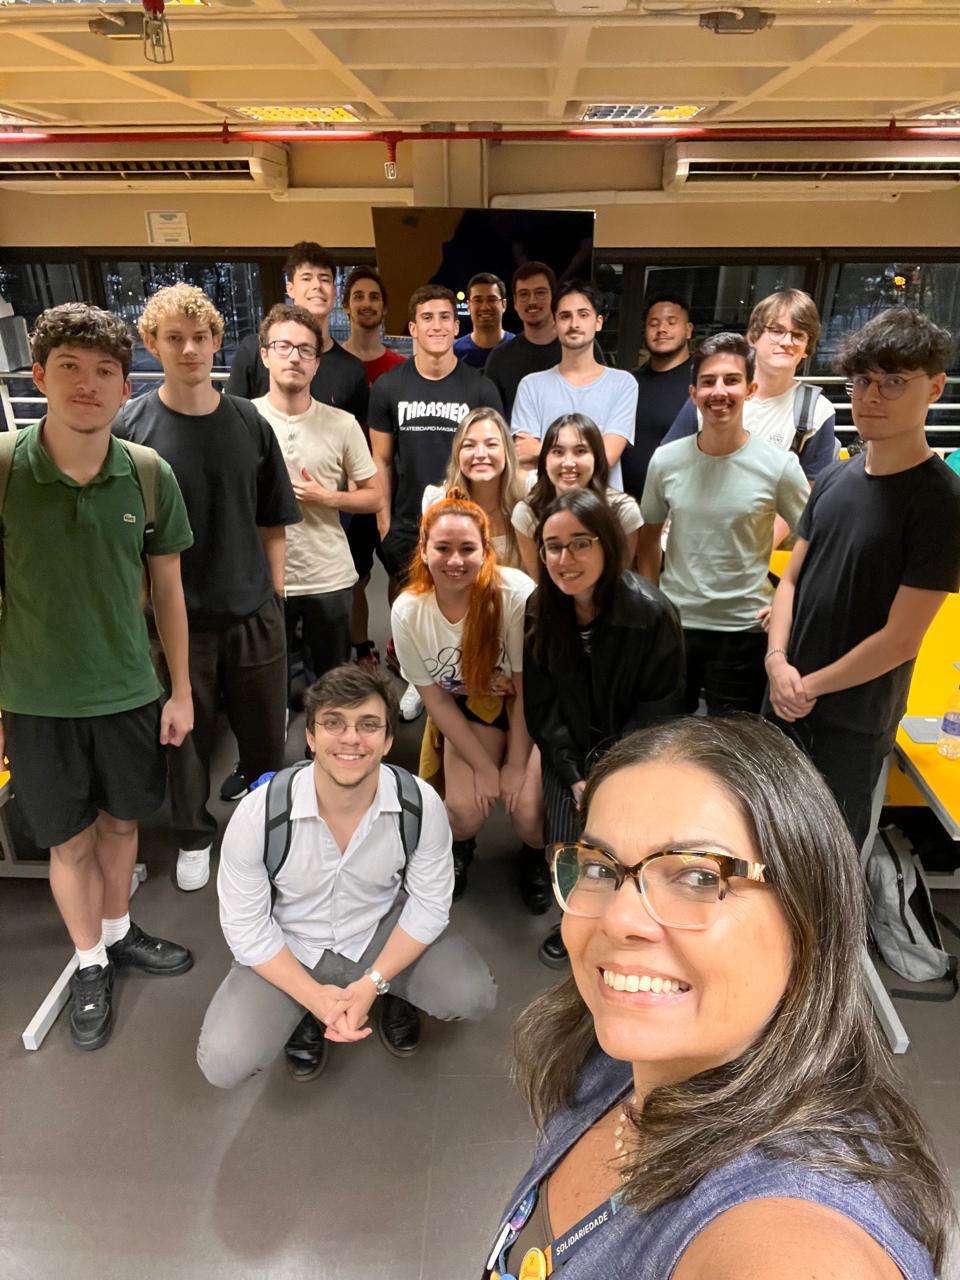
\includegraphics[width=1\linewidth]{conteudo//4 - ages III//conteudo//figures/vango-time.png}
    Fonte: Wiki do Projeto
    \label{fig:projeto-time-vango}
\end{figure}
